\section{Time complexity}
We will now look into the time complexity of our program. If we look at the flowchart to use as a general guide, then we will look into the complexity of each part of our program. We assume that we always work on a constant number of teams, but the amount of days we need to schedule might vary.

\begin{figure}[ht!]
    \centering
    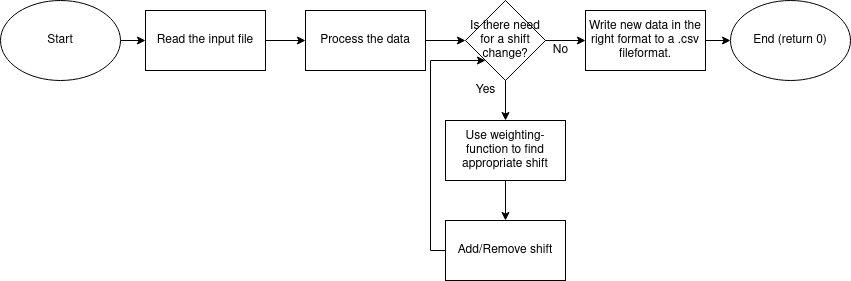
\includegraphics[width=\textwidth]{media/Flowcharts/General Flowchart.png}
    \caption{Flowchart of the program flow.}
    \label{fig:Main_Flowchart2}
\end{figure}

\subsection{Input and output}
Reading the Input file, as shown in the flowchart, is the first step our program goes through. This part has a linear time-complexity, as for each extra day we need to schedule, we have to read another line, and therefore the time used increase. The processing of the data is also linear, as for each day it has to enter the information read into a time slot. Writing out the data to the output file will also have a linear time-complexity, as for each day we need to print some extra information out.

\subsection{The Main Loop}
The main loop is the primary part of our program. We will look into each part of the loop, and then the complexity of the whole.

\subsubsection{Shift Checking}
for each team this function compares the number of hours expected to the number of hours scheduled. Because we assume that we always work on the same number of teams, then this function has a constant time to run, as two numbers for each team just need to be compared.

\subsubsection{Weighing}
The weighing function is the function with the worst time-complexity in our program. This is because for each day we need to check the distance to SH-days, meaning that if more days are added, then for each time slot we potentially need to check more days. This means that the worst case time-complexity of the weighing function is number of days squared. However, because there most likely is going to lie a SH-day at some point, it is only a part of the days that needs to be calculated extra, meaning that the time complexity, although not linear, is not squared.

\subsubsection{Add/Remove shift}
This function also have a constant time complexity, because it simply changes a value of a time slot.


Because the weighing function has a time-complexity that is worse than linear time, the time complexity of the entire program must also be worse than linear. We concluded that the worst case time complexity of the weighing function is the number of days squared. But because the weighing function is in a loop, that also can run op to the number of days, the worst case time complexity of the entire program becomes number of days times number of days squared, or number of days cubed. This worst case will however never occur. For each sh-day, the weighing function will stop before, meaning the average time complexity is much better than number of days squared. Furthermore, it is very unlikely that we need to change every single day, meaning that the loop will not be redone for every single day, making the time complexity even better.

\subsection{Conclusion of time complexity section}
We can conclude that the worst case time complexity of the function is x cubed, but the average time complexity will be much better, as it is very unlikely that we need to make changes to every aspect of the schedule, and all sh-days are removed.


